\begin{figure}[htbp]
\section*{ SMARCC2}
\centering
\begin{subfigure}[b]{0.95\textwidth}
\centering
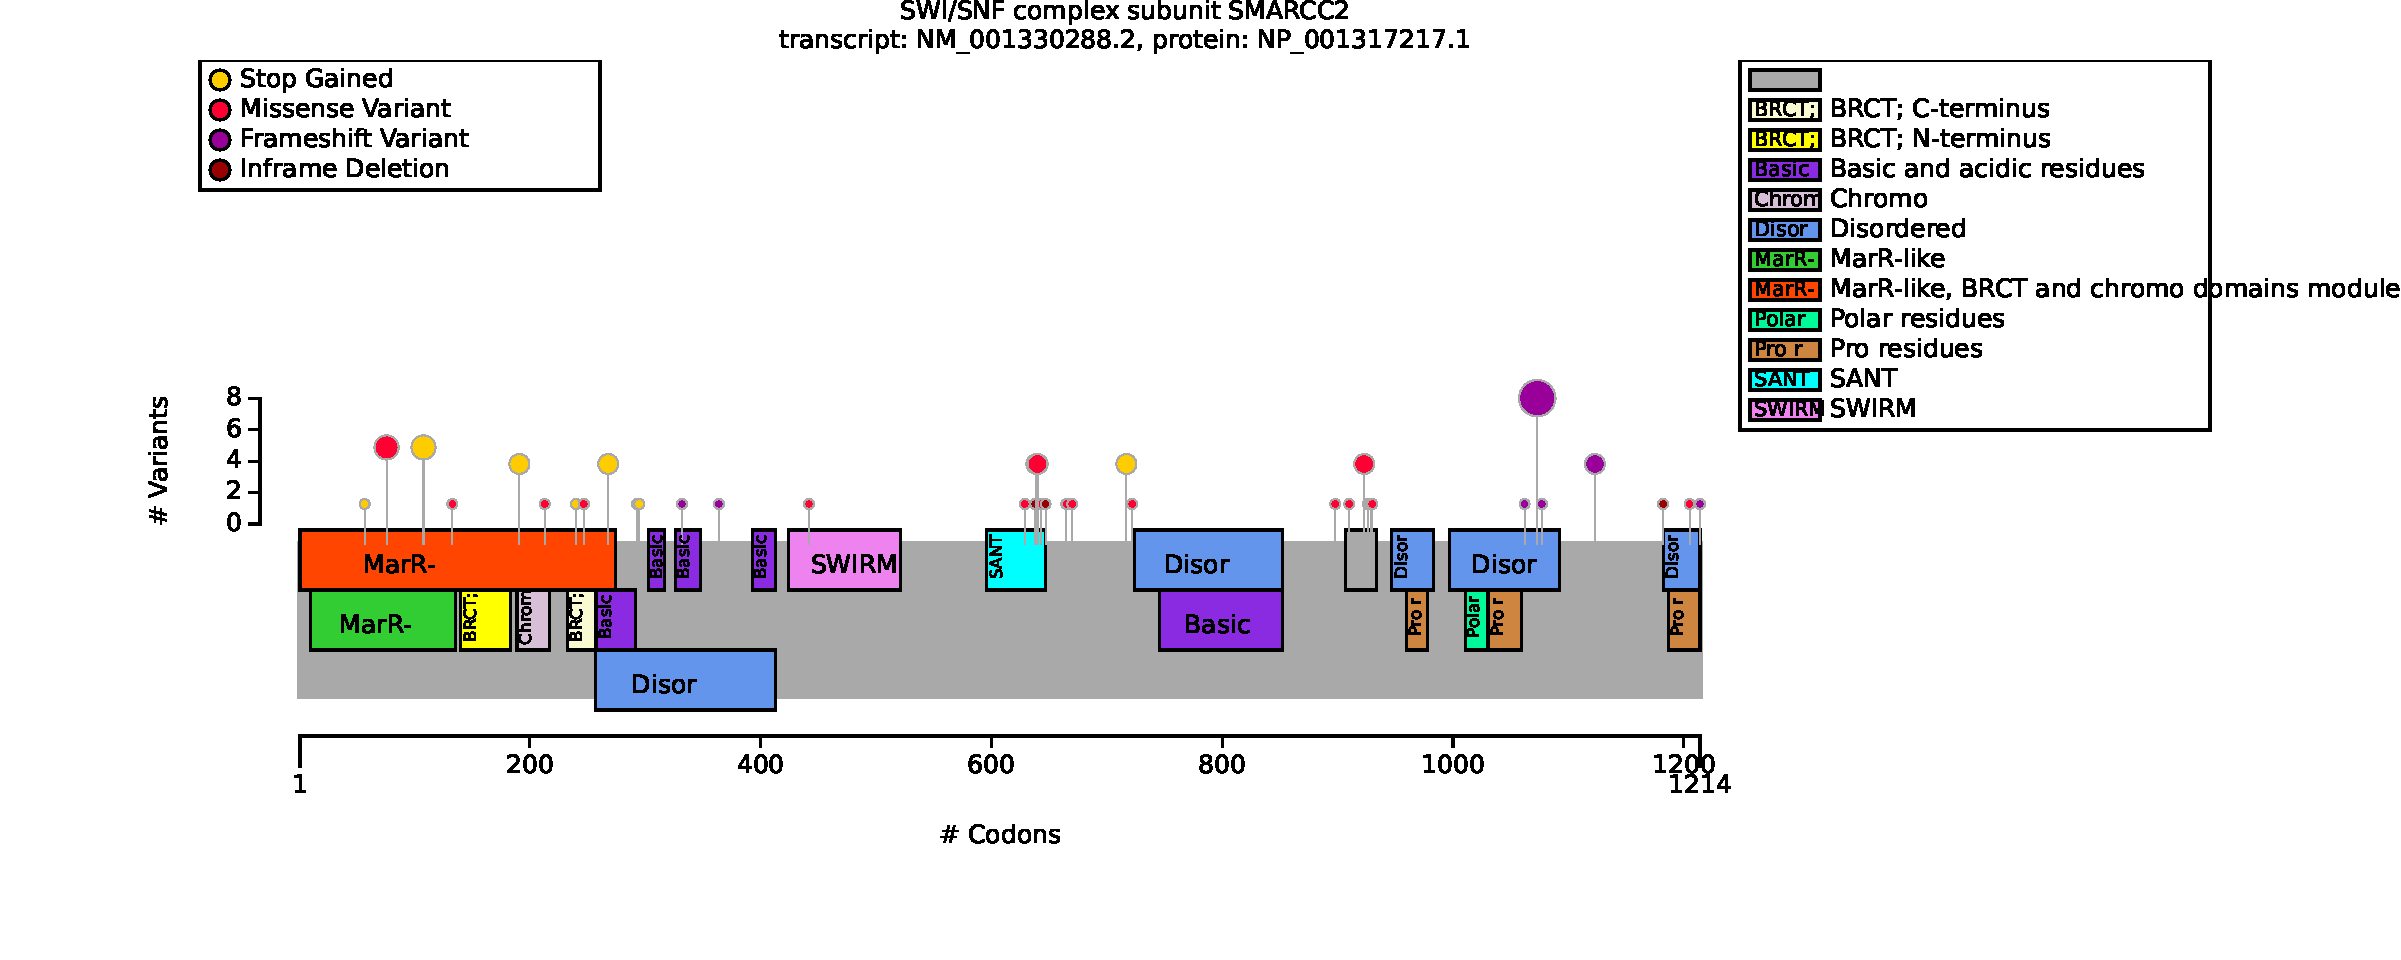
\includegraphics[width=\textwidth]{ img/SMARCC2_protein_diagram-draft.pdf} 
\captionsetup{justification=raggedright,singlelinecheck=false}
\caption{Distribution of variants in SMARCC2}
\end{subfigure}

\vspace{2em}

\begin{subfigure}[b]{0.95\textwidth}
\centering
\resizebox{\textwidth}{!}{
\begin{tabular}{llllrr}
\toprule
HPO term & c.3222del & other & p-value & adj. p-value\\
\midrule
Intellectual disability [HP:0001249] & 1/6 (17\%) & 49/52 (94\%) & $6.99\times 10^{-5}$ & 0.002\\
Autistic behavior [HP:0000729] & 7/8 (88\%) & 13/51 (25\%) & 0.001 & 0.017\\
\bottomrule
\end{tabular}
}
\captionsetup{justification=raggedright,singlelinecheck=false}
\caption{         Fisher Exact Test performed to compare HPO annotation frequency with respect to c.3222del and other. Total of
        24 tests were performed. }
\end{subfigure}
\vspace{2em}
\begin{subfigure}[b]{0.95\textwidth}
\centering
\resizebox{\textwidth}{!}{
\begin{tabular}{llllrr}
\toprule
HPO term & N term & Other & p-value & adj. p-value\\
\midrule
Mild global developmental delay [HP:0011342] & 11/15 (73\%) & 10/43 (23\%) & 0.001 & 0.027\\
\bottomrule
\end{tabular}
}
\captionsetup{justification=raggedright,singlelinecheck=false}
\caption{         Fisher Exact Test performed to compare HPO annotation frequency with respect to N term and Other. Total of
        23 tests were performed. }
\end{subfigure}
\vspace{2em}
\begin{subfigure}[b]{0.95\textwidth}
\centering
\resizebox{\textwidth}{!}{
\begin{tabular}{llllrr}
\toprule
Genotype (A) & Genotype (B) & total tests performed & significant results\\
\midrule
Missense & Truncating & 17 & 0\\
FEMALE & MALE & 26 & 0\\
\bottomrule
\end{tabular}
}
\captionsetup{justification=raggedright,singlelinecheck=false}
\caption{             Fisher Exact Test performed to compare HPO annotation frequency with respect to genotypes. }
\end{subfigure}

\vspace{2em}

\caption{ The cohort comprised 65 individuals (24 females, 37 males, 4 with unknown sex). A total of 118 HPO terms were used to annotate the cohort. Disease diagnosis: Coffin-Siris syndrome 8 (OMIM:618362). to do. A total of 65 unique variant alleles were found in \textit{SMARCC2} (transcript: \texttt{NM\_001330288.2}, protein id: \texttt{NP\_001317217.1}).}
\end{figure}
